%% Преамбула TeX-файла

% 1. Стиль и язык
\documentclass[utf8x]{G7-32} % Стиль (по умолчанию будет 14pt)
\usepackage[T2A]{fontenc}
\usepackage[russian]{babel}

% Остальные стандартные настройки убраны в preamble.inc.tex.
\sloppy

% Настройки стиля ГОСТ 7-32
% Для начала определяем, хотим мы или нет, чтобы рисунки и таблицы нумеровались в пределах раздела, или нам нужна сквозная нумерация.
\EqInChapter % формулы будут нумероваться в пределах раздела
\TableInChapter % таблицы будут нумероваться в пределах раздела
\PicInChapter % рисунки будут нумероваться в пределах раздела

% Добавляем гипертекстовое оглавление в PDF
\usepackage[
bookmarks=true, colorlinks=true, unicode=true,
urlcolor=black,linkcolor=black, anchorcolor=black,
citecolor=black, menucolor=black, filecolor=black,
]{hyperref}

% Изменение начертания шрифта --- после чего выглядит таймсоподобно.
% apt-get install scalable-cyrfonts-tex

\IfFileExists{cyrtimes.sty}
    {
        \usepackage{cyrtimespatched}
    }
    {
        % А если Times нету, то будет CM...
    }

\usepackage{graphicx}   % Пакет для включения рисунков

% С такими оно полями оно работает по-умолчанию:
% \RequirePackage[left=20mm,right=10mm,top=20mm,bottom=20mm,headsep=0pt]{geometry}
% Если вас тошнит от поля в 10мм --- увеличивайте до 20-ти, ну и про переплёт не забывайте:
\geometry{right=20mm}
\geometry{left=30mm}


% Пакет Tikz
\usepackage{tikz}
\usetikzlibrary{arrows,positioning,shadows}

% Произвольная нумерация списков.
\usepackage{enumerate}

% ячейки в несколько строчек
\usepackage{multirow}

% itemize внутри tabular
\usepackage{paralist,array}


% Настройки листингов.
% 8 Листинги

\usepackage{listings}

% Значения по умолчанию
\lstset{
  basicstyle= \footnotesize,
  breakatwhitespace=true,% разрыв строк только на whitespacce
  breaklines=true,       % переносить длинные строки
%   captionpos=b,          % подписи снизу -- вроде не надо
  inputencoding=koi8-r,
  numbers=left,          % нумерация слева
  numberstyle=\footnotesize,
  showspaces=false,      % показывать пробелы подчеркиваниями -- идиотизм 70-х годов
  showstringspaces=false,
  showtabs=false,        % и табы тоже
  stepnumber=1,
  tabsize=4,              % кому нужны табы по 8 символов?
  frame=single
}

% Стиль для псевдокода: строчки обычно короткие, поэтому размер шрифта побольше
\lstdefinestyle{pseudocode}{
  basicstyle=\small,
  keywordstyle=\color{black}\bfseries\underbar,
  language=Pseudocode,
  numberstyle=\footnotesize,
  commentstyle=\footnotesize\it
}

% Стиль для обычного кода: маленький шрифт
\lstdefinestyle{realcode}{
  basicstyle=\scriptsize,
  numberstyle=\footnotesize
}

% Стиль для коротких кусков обычного кода: средний шрифт
\lstdefinestyle{simplecode}{
  basicstyle=\footnotesize,
  numberstyle=\footnotesize
}

% Стиль для BNF
\lstdefinestyle{grammar}{
  basicstyle=\footnotesize,
  numberstyle=\footnotesize,
  stringstyle=\bfseries\ttfamily,
  language=BNF
}

% Определим свой язык для написания псевдокодов на основе Python
\lstdefinelanguage[]{Pseudocode}[]{Python}{
  morekeywords={each,empty,wait,do},% ключевые слова добавлять сюда
  morecomment=[s]{\{}{\}},% комменты {а-ля Pascal} смотрятся нагляднее
  literate=% а сюда добавлять операторы, которые хотите отображать как мат. символы
    {->}{\ensuremath{$\rightarrow$}~}2%
    {<-}{\ensuremath{$\leftarrow$}~}2%
    {:=}{\ensuremath{$\leftarrow$}~}2%
    {<--}{\ensuremath{$\Longleftarrow$}~}2%
}[keywords,comments]

% Свой язык для задания грамматик в BNF
\lstdefinelanguage[]{BNF}[]{}{
  morekeywords={},
  morecomment=[s]{@}{@},
  morestring=[b]",%
  literate=%
    {->}{\ensuremath{$\rightarrow$}~}2%
    {*}{\ensuremath{$^*$}~}2%
    {+}{\ensuremath{$^+$}~}2%
    {|}{\ensuremath{$|$}~}2%
}[keywords,comments,strings]

% Подписи к листингам на русском языке.
\renewcommand\lstlistingname{\cyr\CYRL\cyri\cyrs\cyrt\cyri\cyrn\cyrg}
\renewcommand\lstlistlistingname{\cyr\CYRL\cyri\cyrs\cyrt\cyri\cyrn\cyrg\cyri}


% Полезные макросы листингов.
% Любимые команды
\newcommand{\Code}[1]{\textbf{#1}}


\includeonly{1-linux,2-Zprime,80-conclusion,81-biblio}

\begin{document}

\frontmatter % выключает нумерацию ВСЕГО; здесь начинаются ненумерованные главы: реферат, введение, глоссарий, сокращения и прочее.

% Команды \breakingbeforechapters и \nonbreakingbeforechapters
% управляют разрывом страницы перед главами.
% По-умолчанию страница разрывается.

% \nobreakingbeforechapters
% \breakingbeforechapters

% Также можно использовать \Referat, как в оригинале
\begin{abstract}
Это пример каркаса расчётно-пояснительной записки, желательный к использованию в РПЗ проекта по курсу РСОИ.

Данный опус, как и более новые версии этого документа, можно взять по адресу (\url{https://github.com/rominf/latex-g7-32}).

Текст в документе носит совершенно абстрактный характер.
\end{abstract}

%%% Local Variables: 
%%% mode: latex
%%% TeX-master: "rpz"
%%% End: 


\tableofcontents

\Introduction

Целью работы является создание всякой всячины. Для достижения поставленной цели необходимо решить следующие задачи:

\begin{itemize}
\item проанализировать существующую всячину;
\item спроектировать свою, новую всячину;
\item изготовить всякую всячину;
\item проверить её работоспособность.
\end{itemize}

Вот так-то. А этот абзац вставлен для визуальной оценки отступа от перечня до следующего абзаца.

\mainmatter % это включает нумерацию глав и секций в документе ниже

\chapter{Операционная система Linux: состояние и тенденции развития}
\label{cha:analysis}

\section{Основные операционные системы}

В наше время существует огромное множество типов операционныхсистем, имеющих различные области применения. В таких условиях можновыделить четыре основных критерия, описывающих назначение ОС.

Операционная система (ОС) — комплекс взаимосвязанных программ,предназначенных   для   управления   ресурсами   вычислительного   устройства.Благодаря   этим   программам   происходит   организация   взаимодействия   спользователем.  Управление   памятью,   процессами,   и   всем   программным   иаппаратным обеспечением устраняет необходимость работы непосредственно сдисками и предоставляет простой, ориентированный на работу с файламиинтерфейс,   скрывает   множество   неприятной   работы   с   прерываниями,счетчиками времени, организацией памяти и другими компонентами.~\cite{Oc1}

Организация   удобного   интерфейса,   позволяющая   пользователювзаимодействовать   с  аппаратурой   компьютера   за   счет   некой   расширеннойвиртуальной   машины,   с   которой   удобнее   работать   и   которую   легчепрограммировать.   Вот   перечень   основных   сервисов,   предоставляемыхтипичными операционными системами.Разработка программ, где ОС представляет программисту разнообразныеинструменты разработки приложений: редакторы, отладчики и т.п. Ему необязательно   знать,   как   функционируют   различные   электронные   иэлектромеханические узлы и устройства компьютера. Часто пользователь можетобойтись   только   мощными   высокоуровневыми   функциями,   которыепредставляет ОС.Также, для запуска программы нужно выполнить ряд действий: загрузитьв основную память программу и данные, инициализировать устройства ввода-вывода и файлы, подготовить другие ресурсы. ОС выполняет всю эту работувместо пользователя. ОС дает доступ к устройствам ввода-вывода. Каждое устройство требуетсвой набор команд для запуска. ОС предоставляет пользователю единообразныйинтерфейс,   который   опускает   все   детали   и   дает   программисту   доступ   кустройствам ввода-вывода через простейшие команды чтения и записи. При работе с файлами управление со стороны ОС предполагает не толькоглубокий учет природы устройства ввода-вывода, но и знание структур данных,записанных в файлах. Многопользовательские ОС, кроме того, обеспечиваютмеханизм защиты при обращении к файлам. ОС управляет доступом к совместно используемой или общедоступнойвычислительной системе в целом, а также к отдельным системным ресурсам.Она   обеспечивает   защиту   ресурсов   и   данных   от   несанкционированногоиспользования и разрешает конфликтные ситуации.

Обнаружение ошибок и их обработка— это еще один очень важныймомент   в   назначении   ОС.   При   работе   компьютерной   системы   могутпроисходить разнообразные сбои за счет внутренних и внешних ошибок ваппаратном   обеспечении,   различного   рода   программных   ошибок(переполнение,   попытка   обращения   к   ячейке   памяти,   доступ   к   которойзапрещен и др.). В каждом случае ОС выполняет действия, минимизирующиевлияние ошибки на работу приложения (от простого сообщения об ошибке доаварийной остановки программы).И, наконец, учет использования ресурсов. ОС  имеет средства учетаиспользования   различных   ресурсов   и   отображения   параметровпроизводительности  вычислительной системы. Эта информация важна длянастройки (оптимизации) вычислительной системы с целью повышения еепроизводительности.~\cite{Oc1}

Организация   эффективного   использования   ресурсов   компьютера.   ОСтакже является своеобразным диспетчером ресурсов компьютера. К числуосновных ресурсов современных вычислительных систем относятся основнаяпамять, процессоры,   таймеры, наборы данных, диски, накопители на МЛ,принтеры, сетевые устройства, и др. Перечисленные ресурсы определяютсяоперационной системой между выполняемыми программами. В отличие отпрограммы, которая является статическим объектом, выполняемая программа –это динамический объект, который называется процессом и является базовымпонятием современных ОС. Управление ресурсами вычислительной системы сцелью наиболее эффективного их использования является вторым назначениемоперационной системы. Критерии эффективности, в соответствии с которымиОС организует управление ресурсами компьютера, могут быть различными.Например, в одном случае наиболее важным является пропускная способностьвычислительной систем, в другом – время ее реакции. Зачастую ОС должныудовлетворять   нескольким,   противоречащим   друг   другу   критериям,   чтодоставляет   разработчикам   серьезные   трудности.   Управление   ресурсамивключает решение ряда общих, не зависящих от типа ресурса задач.Планирование ресурса – определение процесса, для которого необходимовыделить ресурс. Здесь предопределяется, когда и в каком качестве долженвыделиться данный ресурс. Удовлетворение запросов на ресурсы – выделениересурсов процессам; мониторинг состояния и учет использования ресурса –поддержание   оперативной   информации   о   задействовании   ресурса   ииспользовании   его   доли.   Разрешение   конфликтов   между   процессами,претендующими на один и тот же ресурс. Для   решения   этих   общих   задач   управления   ресурсами   разные   ОСиспользуют различные алгоритмы, что в итоге и определяет облик ОС в целом,включая   характеристики   производительности,   область   применения   и   дажепользовательский интерфейс.~\cite{Oc1}

Облегчение процессов эксплуатации аппаратных и программных средстввычислительной системы. Ряд операционных систем имеет в своем составенаборы   служебных   программ,   обеспечивающие   резервное   копирование,архивацию данных, проверку, очистку и дефрагментацию дисковых устройств идр. Кроме того, современные ОС имеют достаточно большой набор средств испособов диагностики и восстановления работоспособности системы. Сюдаотносятся: -диагностические программы для выявления ошибок в конфигурацииоперационной системы; -средства восстановления последней работоспособной конфигурации; -средства   восстановления   поврежденных   и   пропавших   системныхфайлов и др.~\cite{Oc1}

Современные   ОС   организуются   таким   образом,   что   допускаютэффективную   разработку,   тестирование   и   внедрение   новых   системныхфункций,   не   прерывая   процесса   нормального   функционированиявычислительной   системы.   Большинство   операционных   систем   постоянноразвиваются (нагляден пример Windows). Происходит это в силу следующихпричин. [1]Для удовлетворения пользователей или нужд системных администраторовОС должны постоянно предоставлять новые возможности. Например, можетпотребоваться   добавить   новые   инструменты   для   контроля   или   оценкипроизводительности,   новые   средства   ввода-вывода   данных   (речевой   ввод).Другой пример – поддержка новых приложений, использующих окна на экранедисплея. [1]В каждой ОС есть ошибки. Время от времени они обнаруживаются иисправляются. Отсюда постоянные появления новых версий и редакций ОС.Необходимость регулярных изменений накладывает определенные требованияна организацию операционных систем. Очевидно, что эти системы должныиметь модульную структуру с четко определенными межмодульными связями.Важную роль играет хорошая и полная документированность системы.~\cite{Oc1}

Функции   ОС   обычно   группируются   либо   в   соответствии   с   типамилокальных   ресурсов,   которыми   управляет   ОС,   либо   в   соответствии   соспецифическими задачами, применимыми ко всем ресурсам. Совокупностимодулей,   выполняющих   такие   группы   функций,   образуют   подсистемыоперационной   системы.   Наиболее   важными   подсистемами   управленияресурсами являются подсистемы управления процессами, памятью, файлами ивнешними устройствами, а подсистемами, общими для всех ресурсов, являютсяподсистемы   пользовательского   интерфейса,   защиты   данных   иадминистрирования.~\cite{Oc2}

Подсистема   управления   процессами   непосредственно   влияет   нафункционирование   вычислительной   системы.   Для   каждой   выполняемойпрограммы ОС организует один или более процессов. Каждый такой процесспредставляется в ОС информационной структурой (таблицей, дескриптором,контекстом   процессора),   содержащей   данные   о   потребностях   процесса   вресурсах, а также о фактически выделенных ему ресурсах (область оперативнойпамяти, количество процессорного времени, файлы, устройства ввода-вывода идр.).   В   современных   мультипрограммных   ОС   может   существоватьодновременно   несколько   процессов,   порожденных   по   инициативепользователей и их приложений, а также инициированных ОС для выполнениясвоих   функций   (системные   процессы).   Поскольку   процессы   могутодновременно претендовать на одни и те же ресурсы, подсистема управленияпроцессами планирует очередность выполнения процессов, обеспечивает ихнеобходимыми   ресурсами,   обеспечивает   взаимодействие   и   синхронизациюпроцессов.~\cite{Oc2}

Подсистема управления памятью производит распределение физическойпамяти   между   всеми   существующими   в   системе   процессами,   загрузку   иудаление программных кодов и данных процессов в отведенные им областипамяти,   а   также   защиту   областей   памяти   каждого   процесса.   Стратегияуправления   памятью   складывается   из   стратегий   выборки,   размещения   изамещения блока программы или данных в основной памяти. Соответственноиспользуются различные алгоритмы, определяющие, когда загрузить очереднойблок в память, в какое место памяти его поместить и какой блок программы илиданных удалить из основной памяти, чтобы освободить место для размещенияновых блоков. Одним из наиболее популярных способов управления памятью всовременных   ОС   является   виртуальная   память.   Реализация   механизмавиртуальной памяти позволяет программисту считать, что в его распоряженииимеется однородная оперативная память, объем которой ограничивается тольковозможностями адресации, предоставляемыми системой программирования.

Нарушения защиты памяти связаны с обращениями процессов к участкампамяти, выделенной другим процессам прикладных программ или программсамой ОС. Средства защиты памяти должны пресекать такие попытки доступапутем аварийного завершения программы-нарушителя.

Функции управления файлами сосредоточены в файловой системе ОС.Операционная система виртуализирует отдельный набор данных, хранящихсяна   внешнем   накопителе,   в   виде   файла   –   простой   неструктурированной последовательности байтов, имеющих символьное имя. Для удобства работы сданными файлы группируются в каталоги, которые, в свою очередь, образуютгруппы – каталоги более высокого уровня. Файловая система преобразуетсимвольные имена файлов, с которыми работает пользователь или программист,в физические адреса данных на дисках, организует совместный доступ кфайлам, защищает их от несанкционированного доступа.  [4]

Функции управления внешними устройствами возлагаются на подсистемууправления внешними устройствами, называемую также подсистемой ввода-вывода.   Она   является   интерфейсом   между   ядром   компьютера   и   всемиподключенными к нему устройствами. Спектр этих устройств очень обширен(принтеры, сканеры, мониторы, модемы, манипуляторы, сетевые адаптеры,АЦП разного рода и др.), сотни моделей этих устройств отличаются набором ипоследовательностью   команд,   используемых   для   обмена   информацией   спроцессором   и   другими   деталями.   Программа,   управляющая   конкретноймоделью внешнего устройства и учитывающая все его особенности, называетсядрайвером. Наличие большого количества подходящих драйверов во многомопределяет   успех   ОС   на   рынке.   Созданием   драйверов   занимаются   какразработчики ОС, так и компании, выпускающие внешние устройства. ОСдолжна поддерживать четко определенный интерфейс между драйверами иостальными   частями   ОС.   Тогда   разработчики   компаний-производителейустройств ввода-вывода могут поставлять вместе со своими устройствамидрайверы для конкретной операционной системы. [4]

Безопасность   данных   вычислительной   системы   обеспечиваетсясредствами отказоустойчивости ОС, направленными на защиту от сбоев иотказов аппаратуры и ошибок программного обеспечения, а также средствамизащиты от несанкционированного доступа. Для каждого пользователя системыобязательна процедура логического входа, в процессе которой ОС убеждается,что в систему входит пользователь, разрешенный административной службой.Корпорация  Microsoft, например, в своем последнем продукте  Windows  10предлагает пользователю вход в систему через распознавание внешности. Этодолжно повысить безопасность и сделать вход в систему быстрее. [6]А вот  Google  обещает нам в новой версии своей ОС для смартфоновAndroid  6.0  доступ   к   устройству  и   подтверждение   покупок   через   сканеротпечатка пальца, если для того пригодно устройство. [7]Администратор   вычислительной   системы   определяет   и   ограничиваетвозможности   пользователей   в   выполнении   тех   или   иных   действий,   т.е.определяет   их   права   по   обращению   и   использованию   ресурсов   системы.Важным средством защиты являются функции аудита ОС, заключающегося вфиксации всех событий, от которых зависит безопасность системы. Поддержкаотказоустойчивости   вычислительной   системы   реализуется   на   основе резервирования   (дисковые   RAID-массивы,   резервные   принтеры   и   другиеустройства, иногда резервирование центральных процессоров, в ранних ОС –дуальные и дуплексные системы, системы с мажоритарным органом и др.).Вообще   обеспечение   отказоустойчивости   системы   –   одна   из   важнейшихобязанностей системного администратора, который для этого использует рядспециальных средств и инструментов.~\cite{Oc2}

Прикладные программисты используют в своих приложениях обращенияк операционной системе, когда для выполнения тех или иных действий имтребуется   особый   статус,   которым   обладает   только   ОС.   Возможностиоперационной   системы   доступны   программисту   в   виде   набора   функций,который называется интерфейсом прикладного программирования (ApplicationProgramming   Interface,  API).   Приложения   обращаются   к   функциям   API   спомощью системных вызовов. Способ, которым приложение получает услугиоперационной   системы,   очень   похож   на   вызов   подпрограмм.   Способреализации   системных   вызовов   зависит   от   структурной   организации   ОС,особенностей аппаратной платформы и языка программирования. В ОС UNIXсистемные вызовы почти идентичны библиотечным процедурам.~\cite{Oc1}

ОС   обеспечивает   удобный   интерфейс   не   только   для   прикладныхпрограмм,   но   и   для   пользователя   (программиста,   администратора,пользователя). На данный момент производители предлагают нам множествофункций, призванных облегчить нашу работу с устройствами и сэкономитьвремя. В качестве примера я опять хочу привести  Windows  10.  Microsoftпомогает   пользователю   обеспечить   беспрепятственную   работу   всех   егоустройств (естественно от  Microsoft) , за счет общей ОС. Тут и мгновеннаяпередача данных с одного устройства на другое, и общие уведомления, которыес такой функцией никак не пропустишь. [6]<<Эффективная, организованная работа>>  – это практически слоган длякаждого производителя ОС. Работа с заметками прямо на веб-страницах, новыемногооконные режимы, несколько рабочих столов – все это мы видим уже какнесколько лет, а у разработчиков еще много идей. [6]

Современные   операционные   системы   имеют   сложную   структуру,состоящую   из   множества   элементов,   где   каждый   из   них   выполняетопределенные функции по управлению процессами и распределению ресурсов.
Ядро ОС – центральная часть операционной системы, обеспечивающаяприложениям   координированный   доступ   к   файловой   системе,   и   обменуфайлами между ПУ. [4]

Командный процессор. Программный модуль ОС, ответственный за чтение отдельных командили же последовательности команд из командного файла, иногда называюткомандным интерпретатором. [4]

Драйверы устройств. К магистрали  компьютера подключаются различные устройства(дисководы,   монитор,   клавиатура,   мышь,   принтер   и   др.).   Каждоеустройство выполняет определенную функцию, при этом техническаяреализация устройств существенно различается. В состав операционнойсистемы входятдрайверы устройств, специальные программы, которыеобеспечивают   управление   работой   устройств   и   согласованиеинформационного обмена с другими устройствами, а также позволяютпроизводить   настройку   некоторых   параметров   устройств.   Каждомуустройству соответствует свой драйвер.[4]

Утилиты. Дополнительные сервисные программы (утилиты) – вспомогательныекомпьютерные   программы   в   составе   общего   программного   обеспечения,делающие   удобным   и   многосторонним   процесс   общения   пользователя   скомпьютером. [4]

Для   удобства   пользователя   в   состав   операционной   системы   обычновходит такжесправочная система. Справочная система позволяет оперативнополучить необходимую информацию как о функционировании операционнойсистемы в целом, так и о работе ее отдельных модулей. [4]



\section{Обзор Linux}
Linux — общее название UNIX-подобных операционных систем на основе одноимённого ядра и собранных для него библиотек и системных программ, разработанных в рамках проекта GNU.
Система UNIX приобрела популярность в связи с ее успешным использованием на мини-ЭВМ. Этот успех послужил толчком к тому, чтобы создать подобную систему и для персональных компьютеров. Как правило, различные версии ОС, относящихся к этому семейству, имеют свои названия, но в основных чертах повторяют особенности UNIX.

GNU/Linux работает на PC-совместимых системах семейства Intel x86, а также на IA-64, AMD64, PowerPC, ARM и многих других.

UNIX - операционная система, которая позволяет осуществить выполнение работ в многопользовательском и многозадачном режиме. Поначалу она предназначалась для больших ЭВМ, чтобы заменить MULTICS. UNIX является очень мощным средством в руках программиста, но требует очень большого объёма ОЗУ и пространства диска. Несмотря на попытки стандартизировать эту операционную систему, существует большое количество различных его версий, главным образом потому, что она была распространена в виде программы на языке Си, которую пользователи стали модифицировать для своих собственных нужд.

\begin{figure}[!h]
	\vspace{0.5cm}
	\begin{center}
	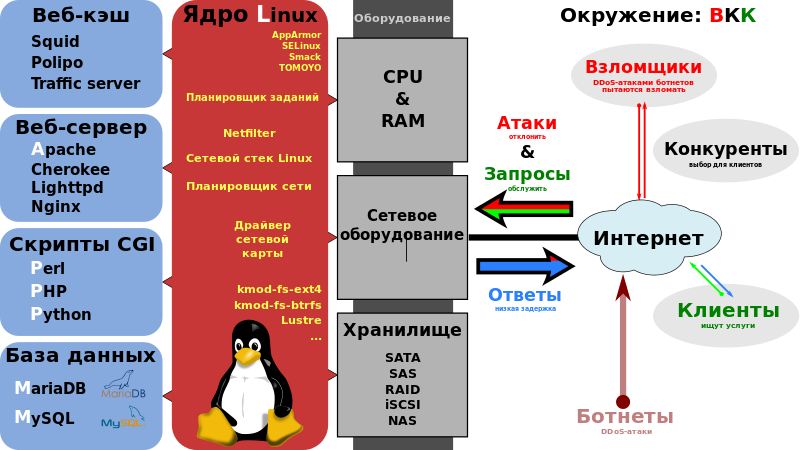
\includegraphics[width=8cm]{figures/LAMP_software_bundle.png}
	\end{center}
	\caption{Структура Linux-системы}
\end{figure}

Очень многие считают, что Linux - это только ядро. Но одно только ядро бесполезно для пользователя. Хотя ядро, несомненно, основа ОС Linux, пользователю все время приходится работать с прикладными программами. Эти программы не менее важны, чем ядро. Поэтому Linux - это совокупность ядра и основных прикладных программ, которые обычно бывают установлены на каждом компьютере с этой операционной системой. Объединение ядра и прикладных программ в единое целое проявляется и в названии системы: GNU/Linux. GNU - это проект по созданию комплекса программ, подобного тому, что обычно сопровождает Unix-подобную систему.

Linux изначально был написан Линусом Торвальдсом, а затем улучшался бесчисленным количеством народа во всем мире. Он является клоном операционной системы Unix, одной из первых мощных операционных систем, разрабатываемых для компьютеров, но не бесплатной. Но ни Unix System Laboratories (создатели Unix), ни Университет Беркли, разработчики Berkeley Software Distribution (BSD), не участвовали в его создании. Один из наиболее интересных фактов из истории Linux'а - это то, что в его создании принимали участие одновременно люди со всех концов света – от Австралии до Финляндии – и продолжают это делать до сих пор.

Дистрибутив – это сама ОС + набор пакетов программ для Linux. Стоит также упомянуть, что все это поставляется с исходными текстами, и любую программу, написанную под Linux, можно переделать под себя. Это же позволяет перенести любую программу на любую платформу – Intel PC, Macintosh. Кстати, все вышеописанное получилось благодаря Free Software Foundation, фонду бесплатных программ, который является частью проекта GNU. И именно для этих целей была создана General Public License (GPL), исходя из которой, Linux – бесплатен, как и весь софт под него, причем коммерческое использование программного обеспечения для Linux или его частей запрещено.

Кроме всего ранее упомянутого, Linux – очень мощная и стабильная ОС. Использование его в Сети оправдывает себя, да и взломать его не так уж и легко.

На сегодняшний день, развитие Linux идет по двум ветвям. Первая, с четными номерами версий(2.0, 2.2, 2.4), считается более стабильной, надежной версией Linux. Вторая, чьи версии нумеруются нечетными номерами(2.1, 2.3), является более дерзкой и быстрее развивающейся и, следовательно (к сожалению), более богатой ошибками.

В Linux нет разделения на диски С, D, и процесс общения с устройствами очень удобен. Все устройства имеют собственный системный файл, все диски подключаются к одной файловой системе и выглядит это все как бы монолитно, едино. Четкая структура каталогов позволяет находить любую информацию мгновенно. Для файлов библиотек – свой каталог, для запускаемых файлов – свой, для файлов с настройками – свой, для файлов устройств – свой, и так далее.

Модульность ядра позволяет подключать любые сервисы ОС без перезагрузки компьютера. Кроме того, вы можете переделать само ядро ОС, благо исходные тексты ядра также имеются в любом дистрибутиве.

В ОС Linux очень умело, если так можно выразиться, используется идея многозадачности, т.е. любые процессы в системе выполняются одновременно (сравните с Windows: копирование файлов на дискету и попытка слушать в этот момент музыку не всегда совместимы).

Linux чуть более сложен, чем Windows, и не всем так просто перейти на него после использования окон. На первый взгляд, может даже показаться, что он очень неудобен и труднонастраиваем.

Linux можно настроить под себя, настроить так, что от пользования этой ОС вы будете испытывать огромное удовлетворение. Огромное количество настроек позволяет изменить внешний (да и внутренний) вид ОС. В Linux есть выбор в использовании графической оболочки, есть несколько офисных пакетов, программы-серверы, файерволы.

В 1998 Linux была самой быстро развивающейся операционной системой для серверов, распространение которой увеличилось в том же году на 212~\%.

Сегодня пользователей Linux насчитывается более 20,000,000. Под Linux существует множество приложений, предназначенных как для домашнего использования, так и для полностью функциональных рабочих станций UNIX и серверов Internet.

Если при использовании коммерческой операционной системы пользователь вынужден ждать выхода следующей версии для того, чтобы получить систему без недостатков предыдущей версии, то модульность Линукса позволяет скачать новое ядро, которое выходит не реже раза в два месяца, а то и чаще (стабильная версия). В Линукс-системах пользователи работают через интерфейс командной строки (CLI), графический интерфейс пользователя (GUI), или, в случае встраиваемых систем, через элементы управления соответствующих аппаратных средств.

Настольные системы, как правило, имеют графический пользовательский интерфейс, в котором командная строка доступна через окно эмулятора терминала или в отдельной виртуальной консоли. Большинство низкоуровневых компонентов Линукс, включая пользовательские компоненты GNU, используют исключительно командную строку.

Командная строка особенно хорошо подходит для автоматизации повторяющихся или отложенных задач, а также предоставляет очень простой механизм межпроцессного взаимодействия. Программа графического эмулятора терминала часто используется для доступа к командной строке с рабочего стола Линукс.

Линукс-системы обычно реализуют интерфейс командной строки при помощи оболочки операционной системы, которая также является традиционным способом взаимодействия с системой Unix. Дистрибутивы, специально разработанные для серверов, могут использовать командную строку в качестве единственного интерфейса.

На настольных системах наибольшей популярностью пользуются пользовательские интерфейсы, основанные на таких средах рабочего стола как KDE Plasma Desktop, GNOME и Xfce, хотя также существует целый ряд других пользовательских интерфейсов. Самые популярные пользовательские интерфейсы основаны на X Window System (часто просто «X» или «иксы»). «X» предоставляет прозрачность сети и позволяет графическим приложениям, работающим на одном компьютере, отображаться на другом компьютере, на котором пользователь может взаимодействовать с ними.

Другие графические интерфейсы, такие как FVWM, Enlightenment и Window Maker, могут быть классифицированы как простые менеджеры окон X Window System, которые предоставляют окружение рабочего стола с минимальной функциональностью.

Оконный менеджер предоставляет средства для управления размещением и внешним видом отдельных окон приложений, а также взаимодействует с X Window System. Окружение рабочего стола включает в себя оконные менеджеры, как часть стандартной установки: (Metacity для GNOME, KWin для KDE, Xfwm для Xfce с 2010 года), хотя пользователь при желании может выбрать другой менеджер окон.

Linux работает на множестве процессоров различных архитектур, таких как x86, x86-64, PowerPC, ARM, Alpha AXP, SPARC, Motorola 680x0, SuperH, IBM System/390, MIPS, PA-RISC, AXIS CRIS, Renesas M32R, Atmel AVR32, Renesas H8/300, NEC V850, Tensilica Xtensa и многих других.

В отличие от коммерческих систем, таких как Windows или Mac OS X, Linux не имеет географического центра разработки. Нет и организации, которая владела бы этой системой; нет даже единого координационного центра. Программы для Linux — результат работы тысяч проектов. Некоторые из этих проектов централизованы, некоторые сосредоточены в фирмах. Многие проекты объединяют хакеров со всего света, которые знакомы только по переписке. Создать свой проект или присоединиться к уже существующему может любой и, в случае успеха, результаты работы станут известны миллионам пользователей. Пользователи принимают участие в тестировании свободных программ, общаются с разработчиками напрямую, что позволяет быстро находить и исправлять ошибки и реализовывать новые возможности.
\section{Сравнительный анализ Linux, MacOS и Windows}

Главной отличительной чертой \textit{Linux} системы является ее модульность и обширный набор системных программ, которые позволяли создать благоприятную обстановку для пользователей-программистов. Система \textit{UNIX} органически сочетается с языком Си, на котором написано более 90\% ее собственных модулей. Командный язык системы практически совпадает с языком Си, что позволяло очень легко комбинировать различные программы при создании больших прикладных систем.

\textit{UNIX} имеет <<оболочку>>, с которой пользователь непосредственно взаимодействует, и <<ядро>>, которое, собственно, и управляет действиями компьютера. Компьютер выводит в качестве приглашения для ввода команд долларовый знак. Из-за продолжительности пользования этой операционной системы количество команд весьма велико. В добавление к командам по управлению файлами, которые присутствуют в любой операционной системе, UNIX имеет, по крайней мере, один текстовый редактор, а также форматер текста и компилятор языка Си, что позволяет, по мере надобности, модифицировать <<оболочку>>.

От \textit{UNIX} многие другие операционные системы переняли такие функции, как переназначение, канал и фильтр; однако \textit{UNIX} имеет, несомненно, преимущество в том, что она с самого начала разрабатывалась как многопользовательская и многозадачная операционная система. Имена файлов могут иметь 14 знаков, причём в именах файлов различаются заглавные и строчные буквы. Первоначальный набор команд операционной системы расширился до 143 в версии 7.0; в версии \textit{System III} добавилась ещё 71 команда, ещё 25 - в \textit{Berkeley} 4.1 и следующие 114 в \textit{Berkeley} 4.2. Из-за такого обилия команд \textit{UNIX} не относится к самым удобным для пользователя языкам. Работа облегчается, если применять графический пользовательский интерфейс, но поскольку такое количество команд и без того занимает значительный объём памяти, этот интерфейс требует ещё большего объёма памяти и пространства диска.

С тем, что такое операционные системы и их особенностями в целом, мы разобрались, теперь самое время приступить к более детальному, конкретному рассмотрению многообразия ОС, которое обычно начинается с рассмотрения краткой истории появления и развития

Считается, что в появлении Юникса в частности виновата компьютерная игра. Дело в том, что Кен Томпсон непонятно чего ради создал игрушку \textit{<<Space Travel>>}. Он написал ее в 1969 году на компьютере \textit{Honeywell-635}, который использовался для разработки \textit{Multics}. Но фишка в том, что ни вышеупомянутый Honeywell, ни имевшийся в лаборатории General \textit{Electric-645} не подходили для игрушки. И Кену пришлось найти другую ЭВМку - 18-разрядный компьютер \textit{РDР-7}. Кен с ребятами разрабатывал новую файловую систему, дабы облегчить себе жизнь и работу. Ну и решил опробовать свое изобретение на новенькой машине. Опробовал. Весь отдел патентов \textit{Bell Labs} дружно радовался. Томпсону этого показалось мало и он начал ее усовершенствовать, включив такие функции как \textit{inodes}, подсистему управления процессами и памятью, обеспечивающую использование системы двумя пользователями в режиме \textit{TimeSharing} (разделения времени) и простой командный интерпретатор. Кен даже разработал несколько утилит под систему. Собственно, сотрудники Кена еще помнили, как они мучались над ОС \textit{Multics}, поэтому в честь старых заслуг один из них - Брайан Керниган - решил назвать ее похожим именем - \textit{UNICS}. Через некоторое время название сократили до \textit{UNIX} (читается так же, просто писать лишнюю букву настоящим программистам во все времена было лень). ОС была написана на ассемблере. Вот мы и подбираемся к тому, что известно в мире как «Первая редакция \textit{UNIX}». В ноябре 1971 года был опубликован первый выпуск полноценной доки по Юниксу. В соответствии с этим и ОС была названа «Первой редакцией \textit{UNIX}». Вторая редакция вышла довольно быстро - меньше, чем через год. Третья редакция ничем особенным не отличалась. Разве что заставила Дениса Ритчи «засесть за словари», вследствие чего тот написал собственный язык, известный сейчас как \textit{С}. Именно на нём была написана 4-я редакция \textit{UNIX} в 1973 году. В июле 1974 года вышла 5-я версия \textit{UNIX}. Шестая редакция \textit{UNIX} (\textit{UNIX V6}), выпущенная в 1975 году, стала первым коммерчески распространяемым Юниксом. Большая ее часть была написана на Си.

Позже была полностью переписана подсистема управления оперативной и виртуальной памятью, заодно изменили интерфейс драйверов внешних устройств. Все это позволило сделать систему легко переносимой на другие архитектуры и было названо «Седьмая редакция» (\textit{UNIX version 7}). Когда в 1976 году в Университет Беркли попала «шестерка», там возникли местные Юникс-гуру. Одним из них был Билл Джой.

Собрав своих друзей-программистов, Билли начал разработку собственной системы на ядре \textit{UNIX} .Запихнув помимо основных функций кучу своих (включая, компилятор Паскаля), он назвал всю эту сборную солянку \textit{Distribution} (\textit{BSD} 1.0). Вторая версия \textit{BSD} почти ни чем не отличалась от первой. Третья версия \textit{BSD} основывалась на переносе \textit{UNIX Version 7} на компьютеры семейства \textit{VAX}, что дало систему \textit{32/V}, легшую в основу \textit{BSD 3.x.} Ну, и самое главное - при этом был разработан стек протоколов \textit{ТСР/IР}; разработка финансировалась Министерством Безопасности США.

Первая коммерческая система называлась \textit{UNIX SYSTEM III} и вышла она в 1982 году. В этой ОС сочетались лучшие качества \textit{UNIX Version 7}.Далее Юниксы развивались примерно так: во-первых, появились компании, занимавшиеся коммерческим переносом \textit{UNIX} на другие платформы. К этому приложила руку и небезызвестная \textit{Microsoft Corporation}, совместно с \textit{Santa Cruz Operation} произведшая на свет \textit{UNIX}-вариацию под названием \textit{XENIX}, во-вторых,\textit{ Bell Labs} создала группу по развитию Юникса и объявила о том, что все последующие коммерческие версии \textit{UNIX} (начиная с \textit{System V}) будут совместимы с предыдущими.

К 1984-му году был выпущен второй релиз \textit{UNIX System V}, в котором появились: возможности блокировок файлов и записей, копирования совместно используемых страниц оперативной памяти при попытке записи (\textit{сору-on-write}), страничного замещения оперативной памяти и т. д. К этому времени ОС \textit{UNIX} была установлена на более чем 100 тыс. компьютеров.

В 1987-м году выпущен третий релиз \textit{UNIX System V}. Было зарегистрировано четыре с половиной миллиона пользователей этой эпической операционной системы. Что касается \textit{Linux}, то он возник лишь в 1990 году, а первая официальная версия ОС вышла лишь в октябре 1991 . Как и \textit{BSD}, \textit{Linux} распространялся с исходниками, чтобы любой пользователь мог настроить ее себе так, как ему хочется. Настраивалось практически всё, чего не может себе позволить, например, \textit{Windows 9x}.

% MacOS

Разработчиком \textit{MacOS} является фирма \textit{Apple} - законодатель мод в области \textit{GUI}, начиная с 1980-х гг. Ключевой идеей \textit{MacOS} с самого начала является разработка и развитие ОС только на основе графического пользовательского интерфейса - <<ОС без командной строки>>. Аппаратная платформа \textit{MacOS} – всевозможные семейства компьютеров \textit{Macintosh} фирмы \textit{Apple} (наиболее популярные среди рабочих станций в США), а также \textit{PowerPC} – рабочая станция \textit{RISC}-архитектуры, совместно разработанная \textit{Apple}, \textit{IBM} и \textit{HP}. Диалекты (версии) \textit{MacOS} различаются по своему подходу к реализации, хотя для пользователя, благодаря удобному графическому интерфейсу, эти различия могут быть незаметны. Класическая \textit{MacOS} (\textit{classic MacOS}) - оригинальная разработка фирмы \textit{Apple}; новая линия \textit{MacOS X} – развитие ОС \textit{MacOS Classic} и ОС \textit{NeXTSTEP} (\textit{UNIX}-подобной ОС), т.е. она является \textit{UNIX}-совместимой.

Для компьютеров \textit{Macintosh} характерен способ соединения устройств \textit{Apple Desktop bus} (сокращённо \textit{ADB}) – специальный вид соединений для подключения мыши, клавиатуры и джойстика к компьютеру. При его использовании все устройства могут соединятся между собой, и только одно следует подключить к машине непосредственно. Такой способ подключения называется цепочкой. Также возможно последовательное соединение (\textit{Daisy chaning}) ряда дополнительных устройств, таких как проигрыватель компакт-дисков, жёсткий диск и сканер.

\textit{Macintosh}-машины имеют встроенную поддержку звука и возможность подключения к сети, а также обеспечивают функцию «включи и работай» (\textit{plug and play}), т.е. при подключении нового оборудования необходимо только произвести его наладку и согласовать с имеющимся. Компьютеры \textit{Macintosh Power} или \textit{Macintosh AV} при помощи адаптера \textit{Geo Port} соединяются непосредственно с телефонной линией, позволяя связываться с оперативными службами, получать и передавать факсы без использования модема.

Персональные компьютеры \textit{Macintosh} представлены несколькими видами. Компактные (моноблочные) модели целиком находятся в одном корпусе. Они могут иметь встроенный или внешний винчестер, у них четкие, но малые по размеру экраны, не отображающие цвета или полутона, мало оперативной памяти и нет гнезд для плат расширения. Модульные Macintosh, в отличии от компактных, состоят из нескольких частей или модулей. Все процессорные блоки у таких моделей имеют одно или несколько гнезд расширения (слотов). Мобильные (портативные) \textit{Macintosh} типа \textit{Power book} представляют собой миниатюрные, легко транспортируемые модели. Небольшие размеры машин этой серии, однако, ограничивают возможности и могут способствовать медленной работе. Вместо мышки (mouse) мобильные модели имеют встроенные шаровые манипуляторы – колобки (\textit{trackball}) или чувствительную к перемещению пальца площадку – сенсорный планшет или пятачок (\textit{trackpad}), что позволяет экономить место.

С момента выпуска первого компьютера \textit{Macintosh} в 1984 году на всех машинах этого семейства и совмещенных с ними используется операционная система \textit{Mac OS}, которая, конечно, может быть дополнена. Параметры её варьируются от версии к версии. Для функционирования компьютера наиболее необходимой является «Системная Папка» (\textit{System Folder}), которая содержит всю основную информацию, задающую систему \textit{Mac Os}. В ней находятся \textit{System file}, \textit{Finder}, шрифты, реквизиты (прикладные мини-программы, а также другие часто используемые программы), принтерные шрифты и т.д., она всегда выделяется особой пиктограммой. Из неё можно легко установить необходимые программы.


% Windows

\textit{Windows} была, наверное, первой операционной системой, которую Биллу Гейтсу никто не заказывал, а разрабатывать ее он взялся на свой страх и риск. Что в ней такого особенного? Во-первых, графический интерфейс. Такой на тот момент был только у пресловутой \textit{Мас OS}. Во-вторых, многозадачность. В общем, в ноябре 1985 вышла \textit{Windows} 1.0. Основной платформой ставились 286-е машины.

Ровно через два года, в ноябре 87-го вышла \textit{Windows} 2.0, через полтора года вышла 2.10. Ничего особенного в них не было. И вот, наконец, революция! Май 1990-го года, вышла \textit{Windows} 3.0. Чего там только не было: и ДОС-приложения выполнялись в отдельном окне на полном экране, и \textit{Сору-Paste} работал для обмена с данными ДОС - приложений, и сами \textit{Windows} работали в нескольких режимах памяти: в реальном (базовая 640 Кб), в защищенном и расширенном. При этом можно было запускать приложения, размер которых превышает размер физической памяти. Имел место быть и динамический обмен данными (\textit{DDE}). Через пару лет вышла и версия 3.1, в которой уже отсутствовали проблемы с базовой памятью. Также была введена новомодная функция, поддерживающая шрифты \textit{True Туре}. Обеспечена нормальная работа в локальной сети. Появился \textit{Drag\&Drop} (перенос мышкой файлов и директорий). В версии 3.11 была улучшена поддержка сети и введено еще несколько малозначительных функций. Параллельно вышла \textit{Windows NT} 3.5, которая была на тот момент сбором основных сетевых примочек, взятых из \textit{OS/2}. В июне 1995 вся компьютерная общественность была взбудоражена сообщением Microsoft о релизе в августе новой операционной системы, существенно иной, нежели \textit{Windows} 3.11.

24 августа -- дата официального релиза \textit{Windows} 95 (другие названия: \textit{Windows} 4.0, \textit{Windows Chicago}).Теперь это была не просто операционная среда -- это была полноценная операционная система. 32-битное ядро позволяло улучшить доступ к файлам и сетевым функциям. 32-битные приложения были лучше защищены от ошибок друг друга, имелась и поддержка многопользовательского режима на одном компьютере с одной системой. Множество отличий в интерфейсе, куча настроек и улучшений.

Чуть позже вышла новая \textit{Windows NT} с тем же интерфейсом, что и 95-е. Поставлялась в двух вариантах: как сервер и как рабочая станция. Системы \textit{Windows NТ 4.x} были надежны, но не столько потому, что у \textit{Microsoft} проснулась совесть, сколько потому, что \textit{NТ} писали программисты, когда-то работавшие над \textit{VАХ/VMS}.


\section{Семейство Linux систем}

К операционной системе \textit{GNU/Linux} также часто относят программы, дополняющие эту операционную систему, и прикладные программы, делающие её полноценной многофункциональной операционной средой. В отличие от большинства других операционных систем, \textit{GNU/Linux} не имеет единой «официальной» комплектации. Вместо этого \textit{GNU/Linux} поставляется в большом количестве так называемых дистрибутивов, в которых программы \textit{GNU} соединяются с ядром \textit{Linux} и другими программами.

В отличие от \textit{Microsoft Windows}, \textit{Mac OS} и коммерческих UNIX-подобных систем, \textit{GNU/Linux} не имеет географического центра разработки. Нет и организации, которая владела бы этой системо, нет даже единого координационного центра. Программы для \textit{Linux} — результат работы тысяч проектов. Некоторые из этих проектов централизованы, некоторые сосредоточены в фирмах. Многие проекты объединяют хакеров со всего света, которые знакомы только по переписке. Создать свой проект или присоединиться к уже существующему может любой и, в случае успеха, результаты работы станут известны миллионам пользователей. Пользователи принимают участие в тестировании свободных программ, общаются с разработчиками напрямую, что позволяет быстро находить и исправлять ошибки и реализовывать новые возможности.

Именно такая гибкая и динамичная система разработки, невозможная для проектов с закрытым кодом, определяет исключительную экономическую эффективность \textit{GNU/Linux}. Низкая стоимость свободных разработок, отлаженные механизмы тестирования и распространения, привлечение людей из разных стран, обладающих разным видением проблем, защита кода лицензией \textit{GPL} — всё это стало причиной успеха свободных программ.

Конечно, такая высокая эффективность разработки не могла не заинтересовать крупные фирмы, которые стали открывать свои проекты. Так появились \textit{Mozilla} (\textit{Netscape, AOL}), \textit{OpenOffice.org} (\textit{Sun}), свободный клон \textit{Interbase} (\textit{Borland}) — \textit{Firebird, SAP DB} (\textit{SAP}). \textit{IBM} способствовала переносу \textit{GNU/Linux} на свои мейнфреймы.

С другой стороны, открытый код значительно снижает себестоимость разработки закрытых систем для \textit{GNU/Linux} и позволяет снизить цену решения для пользователя. Вот почему \textit{GNU/Linux} стала платформой, часто рекомендуемой для таких продуктов, как \textit{Oracle, DB2, Informix, SyBase, SAP R3, Domino}.

Большинство пользователей для установки \textit{GNU/Linux} используют дистрибутивы. Дистрибутив — это не просто набор программ, а ряд решений для разных задач пользователей, объединённых едиными системами установки, управления и обновления пакетов, настройки и поддержки.~\cite{linuxOffDoc}

Самые распространённые в мире дистрибутивы:
\begin{itemize}

\item[--] \textit{Ubuntu}. Быстро завоевавший популярность дистрибутив, ориентированный на лёгкость в освоении и использовании.

\item[--] \textit{openSUSE}. Бесплатно распространяемая версия дистрибутива SuSE, принадлежащая компании \textit{Novell}. Отличается удобством в настройке и обслуживании благодаря использованию утилиты \textit{YaST}.
\item[--] \textit{Fedora}. Поддерживается сообществом и корпорацией \textit{RedHat}, предшествует выпускам коммерческой версии \textit{RHEL}.

\item[--] \textit{Debian}. Международный дистрибутив, разрабатываемый обширным сообществом разработчиков в некоммерческих целях. Послужил основой для создания множества других дистрибутивов. Отличается строгим подходом к включению несвободного ПО.
\item[--] \textit{Mandriva}. Французско-бразильский дистрибутив, объединение бывших \textit{Mandrake} и \textit{Conectiva}.
\textit{Slackware}. Один из старейших дистрибутивов, отличается консервативным подходом в разработке и использовании.

\item[--] \textit{Gentoo}. Дистрибутив, собираемый из исходных кодов. Позволяет очень гибко настраивать конечную систему и оптимизировать производительность, поэтому часто называет себя мета-дистрибутивом. Ориентирован на экспертов и опытных пользователей.

\item[--] \textit{Archlinux}. Ориентированный на применение самых последних версий программ и постоянно обновляемый, поддерживающий одинаково как бинарную, так и установку из исходных кодов и построенный на философии простоты \textit{«KISS»} (\textit{«Keep it simple, stupid»} / «Не усложняй»), этот дистрибутив ориентирован на компетентных пользователей, которые хотят иметь всю силу и модифицируемость \textit{Linux}, но не в жертву времени обслуживания.
\end{itemize}

Помимо перечисленных, существует множество других дистрибутивов, как базирующихся на перечисленных, так и созданных с нуля и зачастую предназначенных для выполнения ограниченного количества задач.

Каждый из них имеет свою концепцию, свой набор пакетов, свои достоинства и недостатки. Ни один не может удовлетворить всех пользователей, а потому рядом с лидерами благополучно существуют другие фирмы и объединения программистов, предлагающие свои решения, свои дистрибутивы, свои услуги. Существует множество \textit{LiveCD}, построенных на основе \textit{GNU/Linux}, например, \textit{Knoppix}. \textit{LiveCD} позволяет запускать\textit{ GNU/Linux} непосредственно с компакт-диска, без установки на жёсткий диск. Большинство крупных дистрибутивов, включая \textit{Ubuntu}, могут быть использованы как \textit{LiveCD}.

Дистрибутивы \textit{Linux} часто бывают ориентированы на конкретные задачи. Поэтому не получится просто составить список операционных систем и сказать: «они – самые лучшие». Здесь выделены несколько областей использования \textit{Linux} и выбраны те дистрибутивы, у которых есть все шансы стать первыми в своей нише в 2017-м.~\cite{linuxDistr}

Лучший дистрибутив для системных администраторов это \textit{Parrot Linux}. У любого администратора всегда полно работы. Без хорошего набора инструментов его дни – это постоянное испытание на прочность, непрерывная гонка. Однако, существует множество дистрибутивов \textit{Linux}, готовых прийти на помощь. Один из них – \textit{Parrot Linux}. Уверен, он приобретёт серьёзную популярность в 2017-м.

Этот дистрибутив основан на \textit{Debian}, он предлагает огромное количество средств для испытания защищённости систем от несанкционированного доступа. Тут, кроме того, можно найти инструменты из сферы криптографии и компьютерной криминалистики, средства для работы с облачными службами и пакеты для обеспечения анонимности. Есть здесь и кое-что для разработчиков, и даже программы для организации времени. Всё это (на самом деле, там – море инструментов) работает на базе стабильной, проверенной временем системы. В результате получился дистрибутив, отлично подходящий для специалистов по информационной безопасности и сетевых администраторов.

Лучший легковесный дистрибутив \textit{LXLE}.  \textit{LXLE} сочетает в себе достойные возможности и скромные системные требования. Другими словами, это дистрибутив, который занимает мало места, но позволяет полноценно работать на компьютере. В \textit{LXLE} можно найти всё необходимое, характерное для релизов \textit{Linux}, рассчитанных на настольные ПК. Система вполне подойдёт для дома, под её управлением смогут работать не самые новые компьютеры (не говоря уже о вполне актуальных системах).

\textit{LXLE} основана на \textit{Ubuntu} 16.04 (как результат – долговременная техподдержка обеспечена), здесь применяется менеджер рабочего стола \textit{LXDE}, который, за более чем десять лет существования, знаком многим, да и устроен несложно.

После установки \textit{LXDE} у под рукой окажется множество стандартных средств, вроде \textit{LibreOffice} и \textit{Gimp}. Единственно, надо будет самостоятельно установить современный браузер.

Лучший корпоративный серверный дистрибутив \textit{RHEL}. По данным \textit{Gartner}~\cite{linuxOffDoc}, \textit{RHEL} принадлежит 67\% рынка \textit{Linux}-дистрибутивов для крупных организаций, при этом подписка на \textit{RHEL} приносит компании \textit{Red Hat} около 75\% доходов. У такого положения дел много причин. Так, \textit{Red Hat} предлагает корпоративным клиентам именно то, что им нужно, но, кроме этого, компания прикладывает огромные усилия к развитию множества проектов с открытым исходным кодом.

\textit{Red Hat} знает – что такое \textit{Linux}, и что такое – корпоративный сектор. \textit{Red Hat} доверяет немало компаний из списка \textit{Fortune} 500 (например, \textit{ING, Sprint, Bayer Business Services, Atos, Amadeus, Etrade}). Дистрибутив \textit{RHEL} вывел множество разработчиков на новый уровень в областях безопасности, интеграции, управления, в сфере работы с облачными системами.



\section{Нынешнее состояние и тенденции развития}

Важно понимать, что организации выбирают \textit{Linux} из-за фактов, а не из-за таблиц сравнения с другими ОС. Возвращаясь к теме фактов о \textit{Linux}, следует сказать, что Linux действительно является надежной, гибкой и высокоэффективной ОС. Вот характерный пример применения: инженеры, проводящие многие часы за клавиатурой, переходят с \textit{Windows} на \textit{Linux}, раздраженные постоянной необходимостью перезагрузки. Интернет-провайдеры (\textit{ISP}) переходят с \textit{Windows} на \textit{Linux}, из-за лучшей управляемости последнего.

\textit{Windows} с другой стороны, традиционно держала пальму первенства, когда требовалась простота использования, легкость установки, прогнозируемость обслуживания, и количество приложений.

Область распространения \textit{Linux} огромна, гораздо больше чем у вcех других операционных систем. Кроме того, что \textit{Linux} прекрасно работает на обычных домашних и рабочих компьютерах и серверах, существуют адаптации \textit{Linux} к большинству современных процессоров, что позволяет использовать системы с ядром \textit{Linux} в сетевом оборудовании, домашней «умной» технике, роботах, мобильных телефонах, различных портативных устройствах и другом оборудовании, поддерживающем программируемые операции.

В конечном счёте столь широкий круг поддерживаемых устройств означает превосходную переносимость программ. Например, одно и то же приложение зачастую можно запустить с минимальными усилиями и на обычном компьютере, и на мобильном телефоне на базе \textit{Linux}. Для примера: \textit{Windows} и её младший брат \textit{Windows Mobile} являются полностью несовместимыми платформами.

Сейчас \textit{Linux} лучше, чем \textit{Windows} справляется с установкой \textit{plug-and-play} устройств (с простым включением в сеть). Рабочий стол \textit{Linux} можно настроить, чтобы он выглядел не только как \textit{Windows}, но и можно запускать пакеты приложений, которые по функциональности эквивалентны \textit{Microsoft Office}. Реализация новых стандартов и протоколов происходит раньше в \textit{Linux}. Это из-за того, что исходный код легко доступен, «заплаты», для дефектов в аппаратуре, для \textit{Linux} иногда выходят в тот же день.

Современные тенденции в развитии ОС.

На основе опыта использования многих современных ОС, можно выделить следующие основные тенденции в их развитии.
\begin{enumerate}
	
	\item Графические оболочки. Любая современная ОС имеет графический пользовательский интерфейс, причем (по вполне понятным причинам острой конкуренции между фирмами-разработчиками) графические оболочки для всех ОС примерно одинаковы по возможностям. Подчас пользователю трудно сориентироваться, в какой именно ОС он работает, хотя для конечных пользователей (непрограммистов), по-видимому, такая унификация удобна.
	
	\item Поддержка новых сетевых технологий и Web-технологий. Сети и Интернет активно развиваются. Появляются новые стандарты и протоколы – \textit{IPv6}, \textit{HTML} 5 (для облачных вычислений) и т.д. Современные ОС развиваются в направлении поддержки всех новых сетевых технологий.
	
	\item Усиленное внимание к механизмам безопасности и защиты. Во многом благодаря инициативе \textit{Trustworthy Computing}, начатой фирмой \textit{Microsoft} в 2002 г., а также ввиду все усиливающейся киберпреступности, все современные ОС уделяют повышенное внимание безопасности: при просмотре веб-страниц браузеры выполняют их проверку на отсутствие \textit{phishing}; загрузки и инсталляции программ из сети выполняются только с явного согласия пользователя и т.д.
	
	\item Поддержка многопоточности и многоядерных процессоров. Ввиду широкого распространения многоядерных процессоров, все современные ОС имеют библиотеки программ, поддерживающие эту возможность аппаратуры. Именно благодаря многоядерной архитектуре, становится реально возможным параллельное выполнение потоков (\textit{threads}).
	
	\item Поддержка распределенных и параллельных вычислений. Современные ОС имеют в своем составе высокоуровневые библиотеки, позволяющие разрабатывать параллельные алгоритмы решения задач – например, поддерживающие стандарты параллелизма OpenMP и MPI.
	
	\item Виртуализация ресурсов и аппаратуры. Современные ОС имеют в своем составе средства виртуализации, позволяющие выполнять приложения для других платформ в изолированных виртуальных машинах, в которые могут быть инсталлированы другие операционные системы.
	
	\item Развитие файловых систем с целью защиты информации и значительного увеличения размера файлов (для мультимедиа). Современные требования обработки мультимедийной информации приводят к тому, что старые файловые системы (например, \textit{FAT}) оказываются недостаточными для хранения мультимедийных файлов. Например, максимальный размер файла в системе \textit{FAT} – 4 гигабайта – легко может быть превышен при переписи на компьютер цифровой видеопленки длительностью 10-15 минут. Поэтому разрабатываются новые файловые системы, допускающие хранение очень больших файлов, например, система \textit{ZFS} в ОС \textit{Solaris}. Другим требованием является обеспечение конфиденциальности информации, которое приводит к необходимости реализации в файловых системах возможности криптования (которая реализована, например, в файловой системе \textit{ZFS}).
\end{enumerate}

Благодаря открытости и гибкости \textit{Linux} стала идеальной операционной системой для лабораторий и других исследовательских учреждений, находящихся на переднем крае революционных технологических изменений.  Исследования, проводимые в \textit{IBM}, охватывают все области информационных технологий – от физики и когнитологии до передовых прикладных исследований и т.д. Однако ученые корпорации IBM также вовлечены в решение чисто научных проблем.  В \textit{IBM}, так же как и во многих других местах, для этого часто используется \textit{Linux}.

\textit{Linux} легко кластеризируется и настраивается для проведения специфических экспериментов, моделирования, выполнения вычислений или тестов. Кроме того, ученые получают в свое распоряжение огромный объем бесплатных программных средств, для работы с которыми и был создан \textit{Linux}.   Потенциал и перспективы эры компьютеров, в которой мы живем, еще в значительной мере не исчерпаны, несмотря на появление в настоящее время таких выдающихся технологий, как \textit{Grid}-вычисления, приложения для беспроводной передачи голоса, искусственный интеллект и квантовые вычисления. Надежность, открытость и гибкость \textit{Linux} означают, что эта система будет оставаться на переднем плане разработок в течение многих лет.

\chapter{Рождения $ Z^\prime $ - бозонов в протон-протонных столкновениях с учетом эффектов $ Z $ - $ Z^\prime $ смешивания}

\section{Новая физика}

Несмотря на впечатляющий успех в описании экспериментов, Стандартная модель не может считаться окончательной теорией элементарных частиц. У нее есть свои трудности. Физики уверены, что она должна быть частью некоторой более глубокой теории строения микромира, той частью, которая видна в экспериментах на коллайдерах при энергиях ниже примерно 1 ТэВ. Главная задача Большого адронного коллайдера — получить хотя бы первые намеки на то, что это за более глубокая теория.

Теоретики разработали большое число кандидатов на такую теорию. Все они, естественно, включают какие-то элементы, которые отсутствуют в Стандартной модели. Часто такие теории коллективно называют «Новая физика» или «За пределами Стандартной модели». На этой странице перечислены некоторые из активно изучаемых вариантов Новой физики~\cite{2part-1}.

Суперсимметрия — это гипотетическая симметрия между фермионами и бозонами. Теории, использующие эту идею, оказываются удивительно мощными, и потому именно с суперсимметрией многие связывают надежды на открытие физики за пределами Стандартной модели. Однако до сих пор не было получено ни одного убедительного доказательства в пользу того, что суперсимметрия реализуется в нашем мире. Ее поиск является одной из главных задач Большого адронного коллайдера.
\begin{figure}
	\centering
	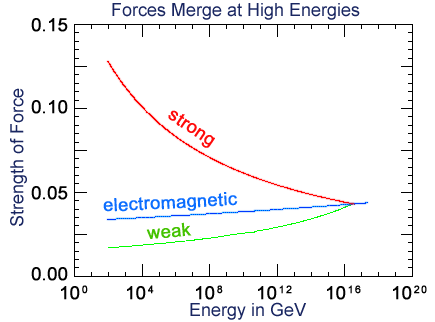
\includegraphics[width=\textwidth]{figures/hep-sm}
	\caption{Константы связи трех взаимодействий частиц}
	\label{fig:fig01}
\end{figure}
Константы связи трех взаимодействий частиц в микромире сходятся к одному значению, если имеющиеся сейчас данные экстраполировать в область очень высоких энергий. Это совпадение считается неслучайным и воспринимается физиками как намек на то, что все три взаимодействия при больших энергиях объединяются в одно.

В XIX веке физики обнаружили, что электричество и магнетизм — это две стороны одной медали, электромагнитного взаимодействия. Век спустя, при создании Стандартной модели, электромагнетизм и слабые ядерные силы были объединены в рамках единого электрослабого взаимодействия. (Точнее говоря, внутри электрослабого взаимодействия имеются по-прежнему две разные силы, а электромагнитное и слабое взаимодействия возникают как комбинации этих сил.) Каждое такое объединение упрощало теорию, уменьшало количество введенных в нее «сущностей», переводило наше понимание микромира на новый уровень.

Сейчас физики имеют сразу несколько причин подозревать, что при очень высоких энергиях происходит объединение электрослабого и сильного взаимодействий (рисунок 2.1). Модели, использующие эту идею (так называемые Теории великого объединения) разрабатываются уже давно. В идеале хотелось бы, чтобы такая теория естественным образом объясняла, почему фундаментальных взаимодействий именно столько и именно с такими свойствами, а также имела четкие предсказания, доступные проверке в современных экспериментах.

При энергиях элементарных частиц, доступных на ускорителях, гравитация по-прежнему остается исключительно слабой, так что заметить ее проявления не удается. Однако ее сила растет с ростом энергии, и при энергиях столкновения порядка планковской она станет столь же важной, как и другие взаимодействия. В этом случае в полный рост встает исключительно сложный вопрос о том, как включить гравитацию в квантовое описание микромира. Поскольку гравитация в современной физике считается проявлением кривизны пространства-времени, успешная теория с сильной гравитацией должна описывать в рамках единого формализма не только все взаимодействия и всё вещество, но и структуру пространства-времени.

Одним из наиболее привлекательных путей решения этого вопроса является теория суперструн и ее дальнейшее развитие в виде теории бран и М-теории. В этих теориях считается, что фундаментальными объектами, существующими в многомерной вселенной, являются не точечные частицы, а протяженные объекты — струны, мембраны и еще более многомерные образования. В этой теории были получены впечатляющие успехи при высоких энергиях, однако при попытке вывести свойства нашего низкоэнергетического мира из теории суперструн возникает обескураживающая неопределенность предсказаний.

Долгое время казалось, что проверка предсказаний теории суперструн лежит далеко за пределами возможностей человечества, поскольку речь идет об энергиях, на 15 порядков превышающих энергии современных ускорителей. Однако примерно 10 лет назад возникло новое направление развития теории, в котором гравитация становится сильной на энергиях порядка 1 ТэВ. Такая возможность возникает в том случае, если наш мир более чем трехмерный и если при этом новые дополнительные пространственные размерности достаточно протяженны: либо они бесконечны, либо свернуты в многомерные петельки размером много больше ядерного масштаба.

В этом случае на LHC следует ожидать целый ряд совершенно замечательных эффектов, отсутствующих в Стандартной модели, например, рождение гравитонов, которые будут улетать из нашего мира в дополнительные измерения, и микроскопических черных дыр, тут же испаряющихся с испусканием множества обычных частиц. Будут также наблюдаться сильные отклонения от предсказаний Стандартной модели в столкновении обычных частиц. Стоит, впрочем, подчеркнуть, что пока нет никаких экспериментальных подтверждений того, что эта красивая гипотеза имеет отношение к нашему миру.

Все три перечисленные выше направления «Новой физики» опираются на глубокие теоретические гипотезы об устройстве нашего мира (суперсимметрия, единство сил, квантово-гравитационная вселенная). Однако кроме этих направлений теоретики также рассматривают разнообразные теории «статусом пониже». В этих теориях просто отмечается, что текущие экспериментальные данные не запрещают те или иные экзотические объекты или явления, и разрабатываются их следствия. Вот несколько примеров таких моделей разной степени экзотичности.

\begin{figure}
	\centering
	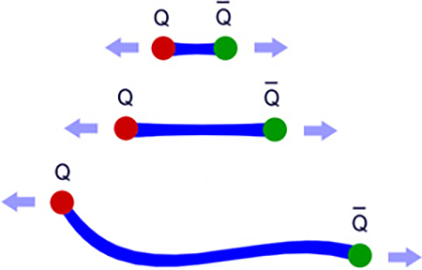
\includegraphics[width=\textwidth]{figures/quirk-antiquirk.jpg}
	\caption{Квирки}
	\label{fig:fig01}
\end{figure}

Неминимальные хиггсовские модели. Поскольку хиггсовские бозоны — единственные частицы Стандартной модели, до сих пор не открытые экспериментально, теоретики изучают самые разные варианты устройства этого сектора теории.
Новые поколения фермионов. Можно предположить, что кроме трех известных поколений кварков и лептонов существуют и другие поколения. Частицы из этих поколений должны быть очень тяжелыми, иначе бы их уже давно открыли в эксперименте.

Новые короткодействующие силы. В таких моделях предполагается, что в нашем мире есть и иные силовые взаимодействия, отличные от сильных, слабых и электромагнитных, но они настолько короткодействующие, что до сих пор никак не проявлялись в эксперименте. На Большом адронном коллайдере благодаря его рекордной энергии удается «прощупать» взаимодействия частиц на исключительно малых расстояниях (менее 10–19 метра), а значит, появляется шанс эти взаимодействия обнаружить. Они могут проявляться либо как рождение и распад частицы-переносчика новых сил (такие гипотетические частицы обозначают Z'), либо как усиленное рассеяние частиц на большие углы.

Лептокварки. В Стандартной модели и в подавляющем большинстве теорий Новой физики кварки и лептоны взаимодействуют друг с другом опосредованно, путем обмена квантами силовых полей. Однако можно представить себе возможность того, что кварки и лептоны исходно являлись фермионами одного типа и лишь потом расщепились на два разных сорта. В таком случае должны существовать новые тяжелые частицы — лептокварки, — которые распадаются прямо на кварк и лептон. Подобные частицы встречаются в теориях Великого объединения.

Квирки. Одним из очень необычных и любопытных вариантов новых сил является гипотеза квирков (quirks). Эта модель построена по типу обычного сильного взаимодействия: в ней предполагается, что существует новое силовое поле с конфайнментом и новые частицы, его чувствующие. Если частицы очень тяжелые, то между ними будут натягиваться длинные, даже макроскопические силовые струны, которые не смогут порваться (рисунок 2.2).





\section{Инструменты имитационного моделирования}



Для исследования отклика детектора на различные физические процессы, созданы программы, позволяющие перевести моделированное на уровне частиц событие  взаимодействия протонов при соударении в формат представления данных детекторов установки \textit{ATLAS}. Алгоритмы моделирования интегрированы в программную оболочку эксперимента  \textit{ATLAS}, именуемую \textit{Athena}, использующую программный пакет \textit{GEANT4}.

Генератор события создает набор частиц, который направляется в программу быстрого или полного моделирования детектора. Генераторы событий встроены в \textit{Athena}. Используется большое число других, поддерживаемых авторами, генераторов, которые имеют блоки связи для использования в \textit{Athena}. Основной массив модельных событий создан с помощью генераторов \textit{PYTHIA}~\cite{2part-pythia-all}, включая его версию \textit{PYTHIAВ},  предназначенную в  \textit{ATLAS} для моделирования событий с рождением \textit{В}-адронов.

\textit{PYTHIA} - это программного пакета для визуализации результатов моделирования процессов столкновения частиц при высоких энергиях осуществляющего генерацию методом Монте-Карло физических событий.

Программы \textit{PYTHIA} интенсивно используются для генерации событий в физике высоких энергий при описании процессов множественного рождения в столкновениях элементарных частиц. В частности задачи, что включает решаемые жесткие с взаимодействия помощью данного в столкновениях $e^+e^-$, $pp$ и $ep$, а также некоторые другие случаи. Программа предназначенна для генерации генератора полных событий, т.е. дают более детальную картину, чем мы наблюдаем в эксперименте, в рамках нашего понимания фундаментальной физики процессов. Обсуждаемые здесь программы Монте-Карло построены как ведомые системы, т.е. пользователь должен написать основную программу. Из нее различные программы вызываются для выполнения частных задач, после чего управление снова передается основной программе. Некоторые из этих задач могут быть весьма тривиальными, и достаточно высокоуровневые программы могут производить большое число вызовов подпрограмм.

Генераторы общего назначения создают событие как целое. Они используют много параметров, часть из которых относится к фундаментальным параметрам, такие как константы связи квантовой хромодинамики (КХД) и электрослабой теории, часть относится к моделям, описывающим взаимодействия на больших расстояниях, с малыми передачами импульса, т.н. «мягкой» КХД, и к электрослабым процессам.

Для корректного моделирования процессов рождения и распада частиц необходимо учитывать условия проведения эксперимента. Это условия рождения изучаемых частиц на ускорителе при соответствующих энергиях сталкивающихся пучков, полные цепочки распадов частиц до уровня <<стабильных частиц>>, регистрируемых детектором. Для решения этих задач применяются генераторы событий, использующие метод Монте-Карло.
Генератор \textit{PYTHIA} является широко используемой в физике высоких энергий программой моделирования столкновений различных частиц в широком диапазоне энергий. Этот генератор учитывает процессы фрагментации кварков в адроны и разыгрывает сложные цепочки адронных распадов. Стартуя с заданного пользователем процесса, (столкновение двух протонов с рождением \textit{Z}-бозона и т.п.) программа случайным образом (с учетом законов сохранения и, по возможности, теоретически известной структуры взаимодействия) разыгрывает конфигурацию конечных партонов, а затем моделирует т.н. процесс адронизации - процесс превращения ненаблюдаемых кварков и глюонов в реальные стабильные и нестабильные частицы с последующим распадом нестабильных частиц. На выходе программа выдает список всех частиц, родившихся в результате столкновения заданных первичных частиц, значения их компонент импульса и энергии. Кроме того, имеется возможность проследить последовательность рождений и распадов от первичного взаимодействия до рождения данной частицы. В качестве входных параметров программы используются описания сталкивающихся частиц, их энергий и тип моделируемого процесса (например, рождение \textit{Z}-бозона). Существующие версии пакета \textit{РYTHIА} написаны на языке программирования \textit{FORTRAN}.
Результаты генерации -- характеристики вторичных частиц -- записываются в файл, что позволяет в дальнейшем проводить статистическую обработку событий.
\section{Распады промежуточных бозонов. Определение массы $Z$-бозона}

В физических программаx экспериментов на  современных  дронных (\textit{LHC}) и планируемых на  электрон-позитронных (\textit{ILC, CLIC}) коллайдерах вопросу поиск  <<новой>> физики, выходящей за  рамки Стандартной модели (СМ), традиционно уделяется большое внимание. К числу подобных теоретических построений, являющихся обобщением СМ, относятся модели с расширенным к либровочным сектором, такие как лево-правосиммет- 
ричные модели (\textit{LR}), альтернативные лево-правосимметричные модели (\textit{ALR}), $E_6$-модели
и др.~\cite{Bobovnikov:2016}. Их исследование (теоретическое и экспериментальное) представляет значи-тельный интерес. Эти модели являются одними из простейших расширений СМ, характеризующихся элементарной структурой хиггсовского сектора. Общим для данных моделей является то, что они предсказывают новые физические объекты и явления на масштабе энергий $O$ (1 ТэВ), связанные, например, с наличием тяжелых нейтральных ($Z^\prime$) калибровочных бозонов, обусловленных дополнительными калибровочными симме-триями $U(1)^\prime$.

Достижение порога рождения $Z^\prime$-бозона явилось бы прямым доказательством про-явления «новой» физики. Однако в данном случае интервал поиска масс $Z^\prime$ ограничен максимальной энергией коллайдера, на котором проводятся эксперименты. Значительно более широкий интервал масс можно исследовать с помощью пропагаторных эффектов. В этом случае ведется поиск отклонений различных наблюдаемых от соответствующих предсказаний СМ. Если экспериментальные данные при достигнутом уровне точности согласуются с СМ, т. е. отклонений от предсказаний СМ нет, то эту экспериментальную информацию можно использовать для получения ограничений на динамические параметры и массы $Z^\prime$-бозонов.

Потенциальные возможности $e^+$$e^-$-коллайдеров для прямого рождения новых калибровочных бозонов гораздо скромнее по сравнению с адронными машинами из-за более низких энергий пучков. Кроме того, современные ограничения на массы $Z^\prime$-бозонов для большинства моделей превосходят планируемую энергию электрон-позитронного коллайдера \textit{ILC}, $\sqrt{s}<< M_{Z^\prime}$. Тем не менее основным достоинством этих машин является возможность проведения экспериментов по измерению наблюдаемых величин с высокой степенью точности и получения однозначной информации о косвенных (виртуальных) эффектах новых $Z^\prime$-бозонов, а также эффектах бозонного $Z$-$Z^\prime$-смешивания. Последние, в моделях с расширенным калибровочным сектором, зависят от структуры хиггсовского сектора модели. Тем самым экспериментальное исследование процессов рождения пар $W^±$-бозонов может не только пролить свет на возможное существование <<новой>> физики, но и дать косвенные указания на хиггсовскую природу, а также установить структуру модели.

На основе данных, полученных из низкоэнергетических экспериментов по нейтральным токам, результатов на $e^+e^-$-коллайдерах \textit{LEP} и \textit{SLC}~\cite{Bobovnikov:2016}, а также недавно выполненных экспериментов по поиску прямого адронного рождения $Z^\prime$-бозонов в процессе Дрелла-Яна.
\begin{center}
	$pp \rightarrow Z^\prime \rightarrow l^+l^- + X$
\end{center}
($l=e,\mu$) на коллайдере \textit{LНC} при энергии $\sqrt{s}$ = 7 и 8 ТэВ с интегральной светимостью соответственно $L_int$ = 5 и 20 фб${}^{-1}$~\cite{Bobovnikov:2016} можно заключить, что для большинства расширенных калибровочных моделей граничные значения для масс дополнительных $Z^\prime$- бозонов находятся в интервале $\sim$ 2,5-3,0 ТэВ (в зависимости от модели), а современный масштаб ограничений на угол смешивания составляет $\mathcal{O}(\varphi )$ ~ ${10}^{-2}$-${10}^{-3}$ рад. При этом наиболее точная информация об угле смешивания была получена преимуще¬ственно из экспериментов на электрон-позитронных коллайдерах \textit{LEP1} и \textit{SLC} по измерению резонансных наблюдаемых физических величин при энергии начальных состояний, равной массе стандартного $Z$-бозона, $\sqrt{s}$ = $M_Z$, в процессах
\begin{center}
	$e^+e^- \rightarrow f\bar{f}$
\end{center}

где конечными фермионными состояниями $f$ были заряженные лептоны и кварки. Высокая точность, достигнутая в экспериментах на коллайдерах \textit{LEP1} и \textit{SLC}, объясняется прежде всего возможностью набора большого объема данных в резонансной области энергии.

Кроме того, эта информация дополнялась данными, полученными на коллайдере тэватрон, по точному измерению массы $M_W$, на основе которых определялся параметр бозонного $Z$−$Z^\prime$-смешивания с использованием соотношения между массами нейтральных и заряженных калибровочных бозонов, $M_Z$ = $M_W$/$(\sqrt{p_0}\cos\theta_W)$, имеющего место в расширенных моделях. Очевидно также, что эти данные будут дополнены новой информацией, которая в ближайшем будущем будет получена в экспериментах на коллайдере \textit{LНС} при энергии 13 и 14 ТэВ. Вместе с тем из этих данных нельзя сделать однозначный вывод о природе «новой» физики, который мог бы вызвать отклонение наблюдаемых величин от их поведения, предсказываемого СМ. Дело в том, что параметр $p$, который содержится в выражениях для векторных и аксиально-векторных констант связи фермионов с учетом петлевых поправок, зависит, в частности, от структуры хиггсовского сектора модели, которая изначально неизвестна. Кроме того, новые тяжелые фермионы и скалярные частицы, предсказываемые моделями с расширенным калибровочным сектором, могут давать вклад в параметр $p$ на петлевом уровне. Все эти неопределенности приводят к появлению систематических (теоретических) погрешностей, которые могут быть весьма существенными при измерении параметра $p$ и, в конечном счете, могут повлиять на точность определения параметра $Z$−$Z^\prime$-смешивания.

Процессы парного рождения заряженных $W^±$-бозонов в адронных столкновениях на \textit{LНС}
\begin{center}
	$pp \rightarrow W^+W^- + X$
\end{center}
электрон-позитронной аннигиляции на \textit{LЕР2} и в большей степени на \textit{ILС}
\begin{center}
	$e^+e^- \rightarrow W^+W^-$
\end{center}

Являются весьма эффективным инструментом поиска эффектов $Z$−$Z^\prime$-смешивания при высоких энергиях и, таким образом, играют роль основного поставщика информации об угле $Z$−$Z^\prime$-смешивания~\cite{Bobovnikov:2016}. С теоретической точки зрения процессы парного рождения заряженных калибровочных бозонов в адронных и электронпозитронных столкновениях интересны тем, что их сечения пропорциональны углу $Z$−$Z^\prime$-смешивания, который, как отмечалось выше, в расширенных калибровочных моделях зависит от структуры хиггсовского сектора.

Прямой поиск тяжелых резонансов в процессе $p\bar{p} \rightarrow W^+W^- + X$ осуществлялся экспериментальными группами \textit{СDF} и \textit{D0} на коллайдере тэватрон. Коллаборация \textit{D0} исследовала возможность рождения резонанса в канале его дибозонного распада, используя чисто лептонные $lvl^\prime v^\prime$ и полулептонные $vjj$ моды. Здесь $l=e,\mu$; $jj$ — две адронные струи. Коллаборация \textit{СDF} также осуществляла поиск тяжелых резонансов в канале их распада в пару заряженных калибровочных бозонов $W^+W^−$ с последующим распадом в полулептонные $evjj$ конечные состояния. Обе коллаборации установили ограничения на массы тяжелых резонансов, таких как новые нейтральные $Z^\prime$- и заряженные калибровочные $W^±$-бозоны, гравитоны Рэндалл-Сандрума. Кроме того, в настоящее время поиск тяжелых резонансов на \textit{LHC} в \textit{WW}-канале интенсивно ведется коллаборациями \textit{ATLAS} и \textit{CMS}. В частности, уже получена экспериментальная информация о процессе в лептонном канале $lvl^\prime v^\prime$ при энергии коллайдера 7 ТэВ и интегральной светимости 4,7 фб${}^{−1}$~\cite{2part-pankov}.

Из анализа экспериментальных данных по измерению процесса электрон-позитронной аннигиляции на коллайдере \textit{LEP2} были впервые получены прямые ограничения на угол $Z$−$Z^\prime$-смешивания. Точность измерения угла смешивания оказалась не очень высокой, $\left |\phi \right |$~5—10 \%, так как сам коллайдер работал в интервале энергий, незначительно превышающем порог реакции, $\sqrt{s} >> 2M_W$. Как было установлено ранее, чувствительность процесса электрон-позитронной аннигиляции к эффектам «новой» физики значительно усиливается при высоких энергиях, $\sqrt{s} >> 2M_W$, где важную роль играет механизм калибровочного сокращения. Дело в том, что вклад $Z^\prime$-бозона в сечение процесса нарушает механизм калибровочного сокращения, играющий важную роль в СМ. Действие механизма калибровочного сокращения состоит в том, что он обеспечивает «правильное» поведение сечения процесса электрон-позитронной аннигиляции с ростом энергии, которое не нарушает унитарный предел, несмотря на быстро растущие с энергией отдельные вклады в сечение. Вместе с тем эффекты, индуцированные появлением дополнительного калибровочного бозона, нарушают механизм калибровочного сокращения в энергетическом интервале $2M_W << \sqrt{s} << M_{Z^\prime}$, что проявляется в виде «разбалансировки» отдельных вкладов в сечение и, как следствие, в возникновении существенно иной по сравнению со СМ энергетической зависимостью сечений. Этим обусловлено действие так называемого механизма усиления эффектов «новой» физики в процессе электрон-позитронной аннигиляции. Именно в силу этого обстоятельства линейный коллайдер \textit{ILC} является одним из основных инструментариев для поиска эффектов «новой» физики при исследовании процесса электрон-позитронной аннигиляции.

Следует отметить также, что коллаборация \textit{CDF} на коллайдере тэватрон одной из первых получила прямые ограничения на угол $Z$−$Z^\prime$-смешивания из обработки данных по измерению процесса адронного рождения $W^+W^−$-бозонов. И вновь относительно небольшая энергия установки и низкая светимость не позволили улучшить ограничения, полученные на коллайдере \textit{LEP2}, а лишь повторить их.

Возможности коллайдера \textit{LНС} по обнаружению эффектов $Z$−$Z^\prime$-смешивания в процессе рождения пар заряженных калибровочных $W^±$-бозонов с их последующим распадом по чисто лептонному каналу $lvl^\prime v^\prime$. Несмотря на очевидное достоинство данного канала, связанное с подавленностью фона, особенно при больших инвариантных массах $W^±$-бозонов, у него имеется заметный недостаток, связанный с присутствием в конечных фермионных состояниях двух нейтрино, что не позволяет восстановить распределение по инвариантной массе бозонных пар из экспериментальных данных. В то же время распад пары $W^±$-бозонов по полулептонному каналу $lvjj$ свободен от указанного недостатка. В процессе $pp \rightarrow Z^\prime \rightarrow WW + X \rightarrow lvjj + X$ существует возможность реконструировать распределение по инвариантной массе $W^+W^-$- пары и тем самым исследовать резонансную структуру $Z^\prime$-бозона. Еще одним достоинством настоящего полулептонного процесса является то, что он имеет сечение, существенно превосходящее сечение чисто лептонного канала. Вместе с тем полулептонный канал, в отличие от лептонного канала $lvl^\prime v^\prime$, имеет большой КХД-фон, вызванный рождением $W_{jj}$-, а также $Z_{jj}$-состояний. В последнем случае предполагается, что $Z$-бозон распадается по лептонному каналу, а в процессе детектирования лептонов один из них теряется. Кроме перечисленных выше КХД фоновых процессов имеется еще один, который играет важную роль в оценке всей фоновой составляющей. Это процесс рождения пар $t\bar{t}$-кварков. Однако большой КХД-фон может быть редуцирован путем наложения кинематических ограничений на поперечные импульсы заряженных лептонов и адронных струй в резонансном сигнале рождения $Z^\prime$-бозонов~\cite{Bobovnikov:2016}.


\chapter{Abc}
\label{cha:analysis}
%
% % В начале раздела  можно напомнить его цель
%
В данном разделе анализируется и классифицируется существующая всячина и пути создания новой всячины. А вот отступ справа в 1 см.~--- это хоть и по ГОСТ, но ведь диагноз же...


% Обратите внимание, что включается не ../dia/..., а inc/dia/...
% В Makefile есть соответствующее правило для inc/dia/*.pdf, которое
% берет исходные файлы из ../dia в этом случае.

\begin{figure}
  \centering
  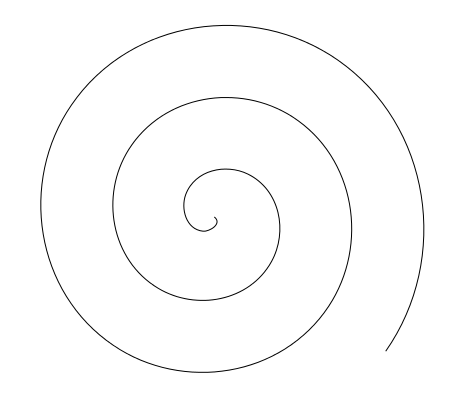
\includegraphics[width=\textwidth]{figures/pic01}
  \caption{Рисунок}
  \label{fig:fig01}
\end{figure}

В \cite{Pup09} указано, что...

Кстати, про картинки. Во-первых, для фигур следует использовать \texttt{[ht]}. Если и после этого картинки вставляются <<не по ГОСТ>>, т.е. слишком далеко от места ссылки,~--- значит у вас в РПЗ \textbf{слишком мало текста}! Хотя и ужасный параметр \texttt{!ht} у окружения \texttt{figure} тоже никто не отменял, только при его использовании документ получается страшный, как в ворде, поэтому просьба так не делать по возможности.

\section{Существующие подходы к созданию всячины}

Известны следующие подходы...

\begin{enumerate}
\item Перечисление с номерами.
\item Номера первого уровня. Да, ГОСТ требует именно так~--- сначала буквы, на втором уровне~--- цифры.
Чуть ниже будет вариант <<нормальной>> нумерации и советы по её изменению.
Да, мне так нравится: на первом уровне выравнивание элементов как у обычных абзацев. Проверим теперь вложенные списки.
\begin{enumerate}
\item Номера второго уровня.
\item Номера второго уровня. Проверяем на длииииной-предлиииииииииинной строке, что получается.... Сойдёт.
\end{enumerate}
\item По мнению Лукьяненко, человеческий мозг старается подвести любую проблему к выбору
  из трех вариантов.
\item Четвёртый (и последний) элемент списка.
\end{enumerate}

Теперь мы покажем, как изменить нумерацию на «нормальную», если вам этого захочется. Пара команд в начале документа поможет нам.

\renewcommand{\labelenumi}{\arabic{enumi})}
\renewcommand{\labelenumii}{\asbuk{enumii})}

\begin{enumerate}
\item Изменим нумерацию на более привычную...
\item ... нарушим этим гост.
\begin{enumerate}
\item Но, пожалуй, так лучше.
\end{enumerate}
\end{enumerate}

В заключение покажем произвольные маркеры в списках. Для них нужен пакет \textbf{enumerate}.
\begin{enumerate}[1.]
\item Маркер с арабской цифрой и с точкой.
\item Маркер с арабской цифрой и с точкой.
\begin{enumerate}[I.]
\item Римская цифра с точкой.
\item Римская цифра с точкой.
\end{enumerate}
\end{enumerate}

В отчётах могут быть и таблицы~--- см. табл.~\ref{tab:tabular} и~\ref{tab:longtable}.
Небольшая таблица делается при помощи \Code{tabular} внутри \Code{table} (последний
полностью аналогичен \Code{figure}, но добавляет другую подпись).

\begin{table}[ht]
  \caption{Пример короткой таблицы с длинным названием на много длинных-длинных строк}
  \begin{tabular}{|r|c|c|c|l|}
  \hline
  Тело      & $F$ & $V$  & $E$ & $F+V-E-2$ \\
  \hline
  Тетраэдр  & 4   & 4    & 6   & 0         \\
  Куб       & 6   & 8    & 12  & 0         \\
  Октаэдр   & 8   & 6    & 12  & 0         \\
  Додекаэдр & 20  & 12   & 30  & 0         \\
  Икосаэдр  & 12  & 20   & 30  & 0         \\
  \hline
  Эйлер     & 666 & 9000 & 42  & $+\infty$ \\
  \hline
  \end{tabular}
  \label{tab:tabular}
\end{table}

Для больших таблиц следует использовать пакет \Code{longtable}, позволяющий создавать
таблицы на несколько страниц по ГОСТ.

Для того, чтобы длинный текст разбивался на много строк в пределах одной ячейки, надо в
качестве ее формата задавать \texttt{p} и указывать явно ширину: в мм/дюймах
(\texttt{110mm}), относительно ширины страницы (\texttt{0.22\textbackslash textwidth})
и~т.п.

Можно также использовать уменьшенный шрифт~--- но, пожалуйста, тогда уж во \textbf{всей}
таблице сразу.

\begin{center}
  \begin{longtable}{|p{0.40\textwidth}|c|p{0.30\textwidth}|}
    \caption{Пример длинной таблицы с длинным названием на много длинных-длинных строк}
    \label{tab:longtable}
    \\ \hline
    Вид шума & Громкость, дБ & Комментарий \\
    \hline \endfirsthead
    \subcaption{Продолжение таблицы~\ref{tab:longtable}}
    \\ \hline \endhead
    \hline \subcaption{Продолжение на след. стр.}
    \endfoot
    \hline \endlastfoot
    Порог слышимости             & 0     &                                                \\
    \hline
    Шепот в тихой библиотеке     & 30    &                                                \\
    Обычный разговор             & 60-70 &                                                \\
    Звонок телефона              & 80    & \small{Конечно, это было до эпохи мобильников} \\
    Уличный шум                  & 85    & \small{(внутри машины)}                        \\
    Гудок поезда                 & 90    &                                                \\
    Шум электрички               & 95    &                                                \\
    \hline
    Порог здоровой нормы         & 90-95 & \small{Длительное пребывание на более
    громком шуме может привести к ухудшению слуха}                                        \\
    \hline
    Мотоцикл                     & 100   &                                                \\
    Power Mower                  & 107   & \small{(модель бензокосилки)}                  \\
    Бензопила                    & 110   & \small{(Doom в целом вреден для здоровья)}     \\
    Рок-концерт                  & 115   &                                                \\
    \hline
    Порог боли                   & 125   & \small{feel the pain}                          \\
    \hline
    Клепальный молоток           & 125   & \small{(автор сам не знает, что это)}          \\
    \hline
    Порог опасности              & 140   & \small{Даже кратковременное пребывание на
    шуме большего уровня может привести к необратимым последствиям}                       \\
    \hline
    Реактивный двигатель         & 140   &                                                \\
                                 & 180   & \small{Необратимое полное повреждение
                                 слуховых органов}                                        \\
    Самый громкий возможный звук & 194   & \small{Интересно, почему?..}                   \\
  \end{longtable}
\end{center}

%%% Local Variables:
%%% mode: latex
%%% TeX-master: "rpz"
%%% End:

\chapter{Конструкторский раздел}
\label{cha:design}

В данном разделе проектируется новая всячина.

\section{Архитектура всячины}

\paragraph{Проверка} параграфа. Вроде работает.
\paragraph{Вторая проверка} параграфа. Опять работает.

Вот.

\begin{itemize}
\item Это список с <<палочками>>.
\item Хотя он и не по ГОСТ, кажется.
\end{itemize}

\begin{enumerate}
\item Поэтому для списка, начинающегося с заглавной буквы, лучше список с цифрами.
\end{enumerate}

Формула \ref{F:F1} совершено бессмысленна.

%Кстати, при каких-то условиях <<удавалось>> получить двойный скобки вокруг номеров формул. Вопрос исследуется.

\begin{equation}
a= cb
\label{F:F1}
\end{equation}


Окружение \texttt{cases} опять работает (см. \ref{F:F2}), спасибо И. Короткову за исправления..


\begin{equation}
a= \begin{cases}
 3x + 5y + z, \mbox{если хорошо} \\
 7x - 2y + 4z, \mbox{если плохо}\\
 -6x + 3y + 2z, \mbox{если совсем плохо}
\end{cases}
\label{F:F2}
\end{equation}

\section{Подсистема всякой ерунды}

Культурная вставка dot-файлов через утилиту dot2tex (рис.~\ref{fig:fig02}).

\begin{figure}
  \centering
% [width=0.5\textwidth] --- регулировка ширины картинки
  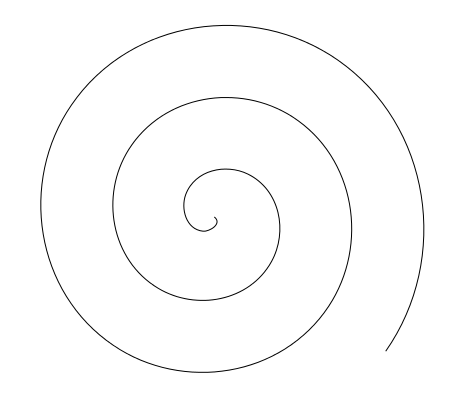
\includegraphics{figures/pic01}
  \caption{Рисунок}
  \label{fig:fig02}
\end{figure}


\subsection{Блок-схема всякой ерунды}

\subsubsection*{Кстати о заголовках}

У нас есть и \Code{subsubsection}. Только лучше её не нумеровать.

%%% Local Variables:
%%% mode: latex
%%% TeX-master: "rpz"
%%% End:

\chapter{Технологический раздел}
\label{cha:impl}

В данном разделе описано изготовление и требование всячины. Кстати,
в Latex нужно эскейпить подчёркивание (писать <<\verb|some\_function|>> для \Code{some\_function}).

\ifPDFTeX
Для вставки кода есть пакет \Code{listings}. К сожалению, пакет \Code{listings} всё ещё
работает криво при появлении в листинге русских букв и кодировке исходников utf-8.
В данном примере он (увы) на лету конвертируется в koi-8 в ходе сборки pdf.

Есть альтернатива \Code{listingsutf8}, однако она работает лишь с
\Code{\textbackslash{}lstinputlisting}, но не с окружением \Code{\textbackslash{}lstlisting}

Вот так можно вставлять псевдокод (питоноподобный язык определен в \Code{listings.inc.tex}):

\begin{lstlisting}[style=pseudocode,caption={Алгоритм оценки дипломных работ}]
def EvaluateDiplomas():
    for each student in Masters:
        student.Mark := 5
    for each student in Engineers:
        if Good(student):
            student.Mark := 5
        else:
            student.Mark := 4
\end{lstlisting}

Еще в шаблоне определен псевдоязык для BNF:

\begin{lstlisting}[style=grammar,basicstyle=\small,caption={Грамматика}]
  ifstmt -> "if" "(" expression ")" stmt |
            "if" "(" expression ")" stmt1 "else" stmt2
  number -> digit digit*
\end{lstlisting}

В листинге~\ref{lst:sample01} работают русские буквы. Сильная магия. Однако, работает
только во включаемых файлах, прямо в \TeX{} нельзя.

% Обратите внимание, что включается не ../src/..., а inc/src/...
% В Makefile есть соответствующее правило для inc/src/*,
% которое копирует исходные файлы из ../src и конвертирует из UTF-8 в KOI8-R.
% Кстати, поэтому использовать можно только русские буквы и ASCII,
% весь остальной UTF-8 вроде CJK и египетских иероглифов -- нельзя.

\lstinputlisting[language=C,caption=Пример (\Code{test.c}),label=lst:sample01]{listings/test.c}

\else

Для вставки кода есть пакет \texttt{minted}. Он хорош всем кроме: необходимости Python (есть во всех нормальных (нет, Windows, я не про тебя) ОС) и Pygments и того, что нормально работает лишь в \XeLaTeX.

Можно пользоваться расширенным BFN:

\begin{listing}[H]
\begin{ebnfcode}
 letter = "A" | "B" | "C" | "D" | "E" | "F" | "G"
       | "H" | "I" | "J" | "K" | "L" | "M" | "N"
       | "O" | "P" | "Q" | "R" | "S" | "T" | "U"
       | "V" | "W" | "X" | "Y" | "Z" ;
digit = "0" | "1" | "2" | "3" | "4" | "5" | "6" | "7" | "8" | "9" ;
symbol = "[" | "]" | "{" | "}" | "(" | ")" | "<" | ">"
       | "'" | '"' | "=" | "|" | "." | "," | ";" ;
character = letter | digit | symbol | "_" ;
 
identifier = letter , { letter | digit | "_" } ;
terminal = "'" , character , { character } , "'" 
         | '"' , character , { character } , '"' ;
 
lhs = identifier ;
rhs = identifier
     | terminal
     | "[" , rhs , "]"
     | "{" , rhs , "}"
     | "(" , rhs , ")"
     | rhs , "|" , rhs
     | rhs , "," , rhs ;
 
rule = lhs , "=" , rhs , ";" ;
grammar = { rule } ;
\end{ebnfcode}
\caption{EBNF определённый через EBNF}
\label{lst:ebnf}
\end{listing}

А вот в листинге \ref{lst:c} на языке C работают русские комменты. Спасибо Pygments и Minted за это.

\begin{listing}[H]
\cfile{inc/src/test.c}
\caption{Пример — test.c} 
\end{listing}
\label{lst:c}

\fi

% Для вставки реального кода лучше использовать \texttt{\textbackslash lstinputlisting} (который понимает
% UTF8) и стили \Code{realcode} либо \Code{simplecode} (в зависимости от размера куска).




Можно также использовать окружение \Code{verbatim}, если \Code{listings} чем-то не
устраивает. Только следует помнить, что табы в нём <<съедаются>>. Существует так же команда \Code{\textbackslash{}verbatiminput} для вставки файла.

\begin{verbatim}
a_b = a + b; // русский комментарий
if (a_b > 0)
    a_b = 0;
\end{verbatim}

%%% Local Variables:
%%% mode: latex
%%% TeX-master: "rpz"
%%% End:

\chapter{Экспериментальный раздел}
\label{cha:research}

В данном разделе проводятся вычислительные эксперименты.
А на рис.~\ref{fig:spire01} показана схема мыслительного процесса автора...

\begin{figure}
  \centering
  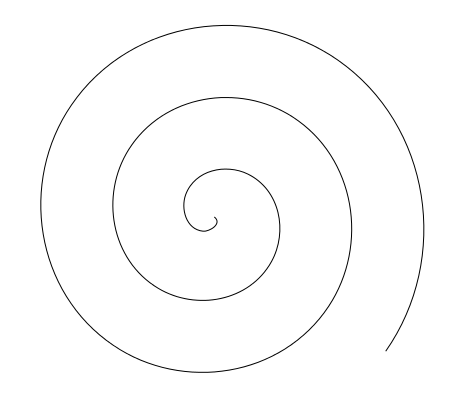
\includegraphics[width=\textwidth]{figures/pic01}
  \caption{Как страшно жить}
  \label{fig:spire01}
\end{figure}


%%% Local Variables:
%%% mode: latex
%%% TeX-master: "rpz"
%%% End:

\Defines % Необходимые определения. Вряд ли понадобться
\begin{description}
\item[Распределённый] Сло123во, которое нельзя употреблять. Но надо протестировать длинные строки в глоссарии.
\end{description}

%%% Local Variables:
%%% mode: latex
%%% TeX-master: "rpz"
%%% End:

\backmatter %% Здесь заканчивается нумерованная часть документа и начинаются ссылки и
            %% заключение

\Conclusion % заключение к отчёту

В результате проделанной работы стало ясно, что ничего не ясно...

%%% Local Variables: 
%%% mode: latex
%%% TeX-master: "rpz"
%%% End: 


% % Список литературы при помощи BibTeX
% Юзать так:
%
% pdflatex rpz
% bibtex rpz
% pdflatex rpz

\bibliographystyle{gost780u}
\bibliography{rpz}

%%% Local Variables: 
%%% mode: latex
%%% TeX-master: "rpz"
%%% End: 


\appendix   % Тут идут приложения

\chapter{Картинки}
\label{cha:appendix1}

\begin{figure}
\centering
\caption{Картинка в приложении. Страшная и ужасная.}
\end{figure}

%%% Local Variables: 
%%% mode: latex
%%% TeX-master: "rpz"
%%% End: 

\chapter{Еще картинки}
\label{cha:appendix2}

\begin{figure}
\centering
\caption{Еще одна картинка, ничем не лучше предыдущей. Но надо же как-то заполнить место.}
\end{figure}

%%% Local Variables: 
%%% mode: latex
%%% TeX-master: "rpz"
%%% End: 


\end{document}

%%% Local Variables:
%%% mode: latex
%%% TeX-master: t
%%% End:
